\documentclass[journal]{IEEEtran}

\usepackage{cite}
\usepackage{amsmath,amssymb,amsfonts}
\usepackage{algorithmic}
\usepackage{graphicx}
\usepackage{textcomp}
\usepackage{xcolor}
\usepackage{booktabs}
\usepackage{multirow}
\usepackage{tabularx}
\usepackage{url}
\usepackage{array}
\usepackage{microtype}
\usepackage{balance}

\newcolumntype{Y}{>{\centering\arraybackslash}X}

\begin{document}

\title{Transformer-Based Data Augmentation and Adaptive Margin Calibration for Low-Resource and Imbalanced Indonesian Text Classification}

\author{\uppercase{Hasan Dwi Cahyono}\IEEEmembership{, Member, IEEE}
\thanks{This research was conducted in the Department of Informatics and Computer Science. Corresponding author: Hasan Dwi Cahyono (e-mail: hasan.dwi.cahyono@gmail.com).}}

\markboth{IEEE Access, Vol. XX, 2026}
{Cahyono: Transformer-Based Data Augmentation and Adaptive Margin Calibration}

\maketitle

\begin{abstract}
Low-resource natural language processing (NLP) for Southeast Asian languages faces persistent challenges stemming from lexical scarcity, informal morphology, and acute class imbalance. Although pretrained transformer encoders such as IndoBERT and IndoBERTweet achieve competitive baseline representations, their performance deteriorates sharply when evaluating multi-class classification tasks characterized by rare, highly ambiguous, or severely skewed label distributions. In this study, we present a comprehensive, multi-phase data augmentation and calibration framework adapted for Bahasa Indonesia. Our architecture leverages autoregressive generative language models (Indonesian GPT-2 decoders) to synthesize synthetic semantic continuations for underrepresented seed classes. To guarantee semantic fidelity and prevent out-of-distribution contamination, synthesized texts undergo multi-metric filtering across four complementary similarity spaces: Sentence-BERT Euclidean distance (ECU), Cosine similarity (COS), lexical Jaccard index (JAC), and Bilingual Evaluation Understudy (BLEU), governed by automated empirical thresholding with strict zero-leakage partitions. Furthermore, to combat minority-class gradient starvation and prior shift without compromising majority-class accuracy, we introduce an automated data-driven calibrator incorporating Fisher-consistent Logit Adjustment ($\tau$-scaled margin shifts), gradient-starvation oversampling, and emoji-semantic lexical mapping combined with heterogeneous multi-model ensembling. We evaluate the proposed pipeline across four distinct Indonesian benchmark benchmarks spanning diverse domains: SmSA (document sentiment), HoASA (aspect-based hotel sentiment with extreme 67.4$\times$ imbalance), EmoT (five-class social emotion), and MovieOpini (conversational film reviews). Extensive empirical evaluations reveal that BLEU and Jaccard filtering deliver statistically significant Macro-F1 enhancements up to $+2.69\%$ on SmSA (elevating neutral F1 from $78.43\%$ to $83.13\%$) and $+16.61\%$ on HoASA, successfully breaking the zero-recall ($0.0\%$ F1) minority barrier while preserving $>94.4\%$ overall accuracy.
\end{abstract}

\begin{IEEEkeywords}
Data augmentation, natural language processing, Bahasa Indonesia, transfer learning, autoregressive language models, logit adjustment, class imbalance, IndoBERT, text classification.
\end{IEEEkeywords}

\section{Introduction}
\label{sec:introduction}

\IEEEPARstart{D}{eep} learning architectures powered by the transformer attention mechanism \cite{vaswani2017attention} have revolutionized natural language understanding (NLU). Pretrained language models (PLMs) such as BERT \cite{devlin2019bert} and RoBERTa \cite{liu2019roberta} serve as ubiquitous foundational backbones for downstream classification tasks, including sentiment analysis, opinion mining, aspect categorization, and emotion recognition. However, the remarkable efficacy of these models fundamentally presupposes the availability of massive, well-curated, and balanced annotated training corpora. 

For languages outside the high-resource anglophone sphere, such as Bahasa Indonesia---the fourth most populous nation's national language spoken by over 270 million people---annotated NLP datasets remain comparatively scarce, domain-fragmented, and intrinsically skewed \cite{wilie2020indonlu, koto2020indolem}. Indonesian text encountered in real-world digital ecosystems (e.g., social media platforms, e-commerce reviews, and community portals) is notoriously characterized by fluid linguistic registers. These include pervasive informal slang (\textit{bahasa gaul}), colloquial clipping, non-standard spelling variants (e.g., \textit{"bgt"} for \textit{"banget"}, \textit{"dgn"} for \textit{"dengan"}), expressive character elongation (e.g., \textit{"senanggg"}), and heavy incorporation of emoji-rich emoticons.

Compounding these lexical complexities is the acute challenge of \textbf{class imbalance}. In practical sentiment and aspect-based classification, real-world data collections rarely exhibit uniform class proportions. In hotel review benchmarks such as HoASA (\textit{Aspect-Based Sentiment Analysis for Airy}) \cite{wilie2020indonlu}, customer feedback is overwhelmingly neutral ($88.61\%$) or mildly positive ($10.07\%$), leaving critical negative service complaints with merely $1.31\%$ representation (only 30 instances in the training partition). In document sentiment corpora like SmSA \cite{purwarianti2019two}, the neutral class comprises only $10.4\%$ of training data compared to $58.3\%$ positive and $31.2\%$ negative, resulting in a severe performance drop where baseline neutral classification F1-scores languish below $78\%$, while positive and negative scores exceed $92\%$. Under standard empirical risk minimization (ERM) optimizing Cross-Entropy loss, deep neural networks are strongly incentivized to minimize global error by collapsing decision margins in favor of the dominant class, resulting in severe false-negative rates and zero-recall blind spots on safety-critical minority samples.

To address sample poverty without prohibitive manual annotation costs, text data augmentation has emerged as a vibrant field of inquiry. Traditional heuristic techniques---such as random token deletion, swapping, synonym substitution via WordNet, and back-translation \cite{wei2019eda, sennrich2016improving}---frequently corrupt semantic coherence, violate syntactic grammar, or alter the ground-truth sentiment polarity in morphologically rich agglutinative languages. Recently, Refai, Abu-Soud, and Abdel-Rahman \cite{refai2023data} demonstrated that autoregressive generative transformers (such as AraGPT2) coupled with multilingual semantic similarity filtering could generate high-fidelity synthetic samples that substantially boost Arabic text classification. 

However, naively transplanting generative augmentation into Indonesian classification exposes three fundamental limitations:
\begin{enumerate}
    \item \textbf{Semantic Drift and Noise Contamination:} Unconstrained causal generation by autoregressive decoders often drifts away from the seed text's core sentiment, hallucinating tangential entities or conflicting polarities that corrupt training sets unless strictly pruned by calibrated multi-metric distance thresholds.
    \item \textbf{Minority Gradient Starvation:} In datasets with extreme imbalance ($IR > 10\times$), naive generation across all underrepresented classes disproportionately allocates generative capacity to moderately frequent classes, leaving ultra-rare classes starved of mini-batch gradient updates during subsequent fine-tuning.
    \item \textbf{Test Prior Shift:} Discrepancies between training and test class distributions (e.g., SmSA's neutral proportion rising from $10.4\%$ in training to $17.6\%$ at test time) cause standard softmax posteriors to produce systematically underconfident and conservative predictions on minority categories.
\end{enumerate}

To overcome these challenges, this paper presents a unified, end-to-end framework integrating generative text augmentation, multi-metric semantic similarity filtering, adaptive logit margin calibration, and heterogeneous multi-model ensembling tailored to Bahasa Indonesia. The principal contributions of this work are summarized as follows:
\begin{itemize}
    \item \textbf{First-Gen and Contemporary Autoregressive Augmentation Pipeline:} We adapt and systematically evaluate causal continuation generation using Indonesian GPT-2 models alongside contemporary lightweight multilingual architectures, generating coherent domain-specific synthetic extensions for minority sentiment seeds.
    \item \textbf{Quad-Metric Semantic Quality Filtering with Zero-Leakage Guarantee:} We establish a rigorous four-dimensional similarity evaluation suite comprising Sentence-BERT Euclidean Distance (ECU), Cosine Similarity (COS), lexical Jaccard index (JAC), and n-gram overlap BLEU scores, combined with strict sample-level hashing to completely prevent data leakage into validation and test sets.
    \item \textbf{Automated Imbalance Calibrator (AIC):} We design a data-driven module that automatically detects class skewness, dynamically calculates Fisher-consistent Logit Adjustment ($\tau$-scaled margins), activates gradient-starvation oversampling multipliers, and adaptively tunes label smoothing regularization without manual hyperparameter search.
    \item \textbf{Emoji-Semantic Normalization and Heterogeneous Ensembling:} We construct an extensive 87-symbol Indonesian emotion mapper converting Unicode emojis and ASCII emoticons into explicit semantic tokens, coupled with a heterogeneous ensemble pipeline combining domain-specialized IndoBERTweet, syntax-grounded IndoBERT-p1, and diverse-vocabulary representations.
    \item \textbf{Exhaustive Benchmark Evaluation:} We conduct rigorous comparative experiments on four benchmark Indonesian datasets (SmSA, HoASA, EmoT, and MovieOpini), evaluating performance through standard Accuracy, Macro-Precision, Macro-Recall, Macro-F1, Balanced Accuracy (BAcc), and multi-class Matthews Correlation Coefficient (MCC).
\end{itemize}

The remainder of this article is organized as follows: Section \ref{sec:related_work} reviews related literature. Section \ref{sec:methodology} delineates the proposed system architecture and mathematical foundations. Section \ref{sec:experimental_setup} details the experimental setup and datasets. Section \ref{sec:results} presents empirical findings and comparative discussions. Section \ref{sec:ablation} provides ablation and sensitivity investigations, and Section \ref{sec:conclusion} concludes the paper.

\section{Related Work}
\label{sec:related_work}

\subsection{Text Data Augmentation in NLP}
Data augmentation in natural language processing is intrinsically more challenging than in computer vision due to the discrete, non-continuous nature of textual tokens where minor alterations can invert semantic truth \cite{shorten2021text}. Early lexical approaches, such as Easy Data Augmentation (EDA) \cite{wei2019eda}, relied on rule-based operations including synonym replacement, random insertion, swap, and deletion. While computationally inexpensive, these heuristics frequently compromise syntax in morphologically complex languages.

Back-translation \cite{sennrich2016improving, edunov2018understanding} leveraged neural machine translation (NMT) pairs to paraphrase sentences, but introduces substantial latency and requires high-quality bilingual models rarely available for low-resource regional dialects. Contextual augmentation using masked language models (MLMs) like BERT \cite{kobayashi2018contextual, wu2019conditional} replaced masked tokens with plausible vocabulary alternatives. However, MLMs are constrained to preserving sentence length and local syntactic structure. 

To expand lexical diversity beyond localized substitutions, generative autoregressive language models have recently gained prominence. Anaby-Tavor et al. \cite{anaby2020not} introduced LAMBADA, demonstrating that fine-tuned GPT-2 decoders can synthesize entire labeled sentences. In the Arabic language sphere, Refai et al. \cite{refai2023data} established that pairing AraGPT2 continuation generation with multilingual sentence embedding distance filtering (Euclidean and Cosine) significantly outstripped traditional augmentation techniques across multiple classification benchmarks. Our research builds upon this foundational paradigm, pioneering its systematic adaptation, extension, and algorithmic enhancement for Bahasa Indonesia.

\subsection{Indonesian Pretrained Language Models}
The release of Indo4B and the IndoNLU benchmark by Wilie et al. \cite{wilie2020indonlu} marked a milestone for Indonesian computational linguistics. The authors introduced IndoBERT (trained on 4 billion words encompassing Indonesian Wikipedia, news portals, and web articles), demonstrating state-of-the-art performance across 12 downstream classification, sequence labeling, and sequence-to-sequence tasks. Subsequently, Koto et al. \cite{koto2020indolem} released IndoLEM and IndoBERTweet, the first large-scale model pre-trained specifically on Indonesian Twitter corpora comprising 409 million tokens. IndoBERTweet demonstrated superior capability in resolving colloquial registers, abbreviations, and informal grammatical structures. Cahya et al. further contributed pretrained BERT, RoBERTa, and GPT-2 models trained on curated Indonesian Wikipedia corpora. While these encoders establish strong sentence representations, their fine-tuning performance remains profoundly vulnerable to extreme minority class starvation, a vulnerability this study directly remediates.

\subsection{Handling Severe Class Imbalance}
Traditional remedies for class imbalance divide into data-level techniques (random oversampling, undersampling, SMOTE \cite{chawla2002smote}) and algorithm-level cost-sensitive loss modifications \cite{cui2019class, lin2017focal}. In NLP, standard oversampling leads to catastrophic overfitting on duplicated samples, while undersampling discards valuable majority data.

Algorithmically, Weighted Cross-Entropy (WCE) penalizes minority misclassifications via static inverse class frequencies, but often causes optimization instability when class ratios exceed $10\times$. Focal Loss \cite{lin2017focal} suppresses gradients from easy samples via a dynamic modulating factor $(1-p_t)^\gamma$. However, as demonstrated by Guo et al. \cite{guo2017calibration}, Focal Loss damages softmax probability calibration and over-indexes on noisy, ambiguous social media labels.

To establish theoretical consistency, Menon et al. \cite{menon2020long} proposed \textbf{Logit Adjustment}. By explicitly enforcing class-prior-dependent margins $\tau \log \pi_y$ directly into network logits prior to softmax normalization, Logit Adjustment is mathematically proven to be Fisher-consistent for minimizing balanced classification error. Cao et al. \cite{cao2019learning} introduced LDAM (Label-Distribution-Aware Margin), enforcing margins scaled inversely with $N_y^{1/4}$. In this study, we operationalize Logit Adjustment within a fully automated, adaptive multi-GPU training pipeline tailored for imbalanced text classification.

\section{Methodology and Architecture}
\label{sec:methodology}

The overall architecture of the proposed Indonesian data augmentation and adaptive classification framework is illustrated in Fig. \ref{fig:architecture}. The pipeline operates across four sequential, tightly coupled phases: (1) Lexical Preprocessing and Emoji Normalization, (2) Autoregressive Continuation Generation, (3) Multi-Metric Semantic Filtering and Strict Leakage Purging, and (4) Adaptive Imbalance Calibration with Multi-Model Classification.

\begin{figure*}[!t]
\centering
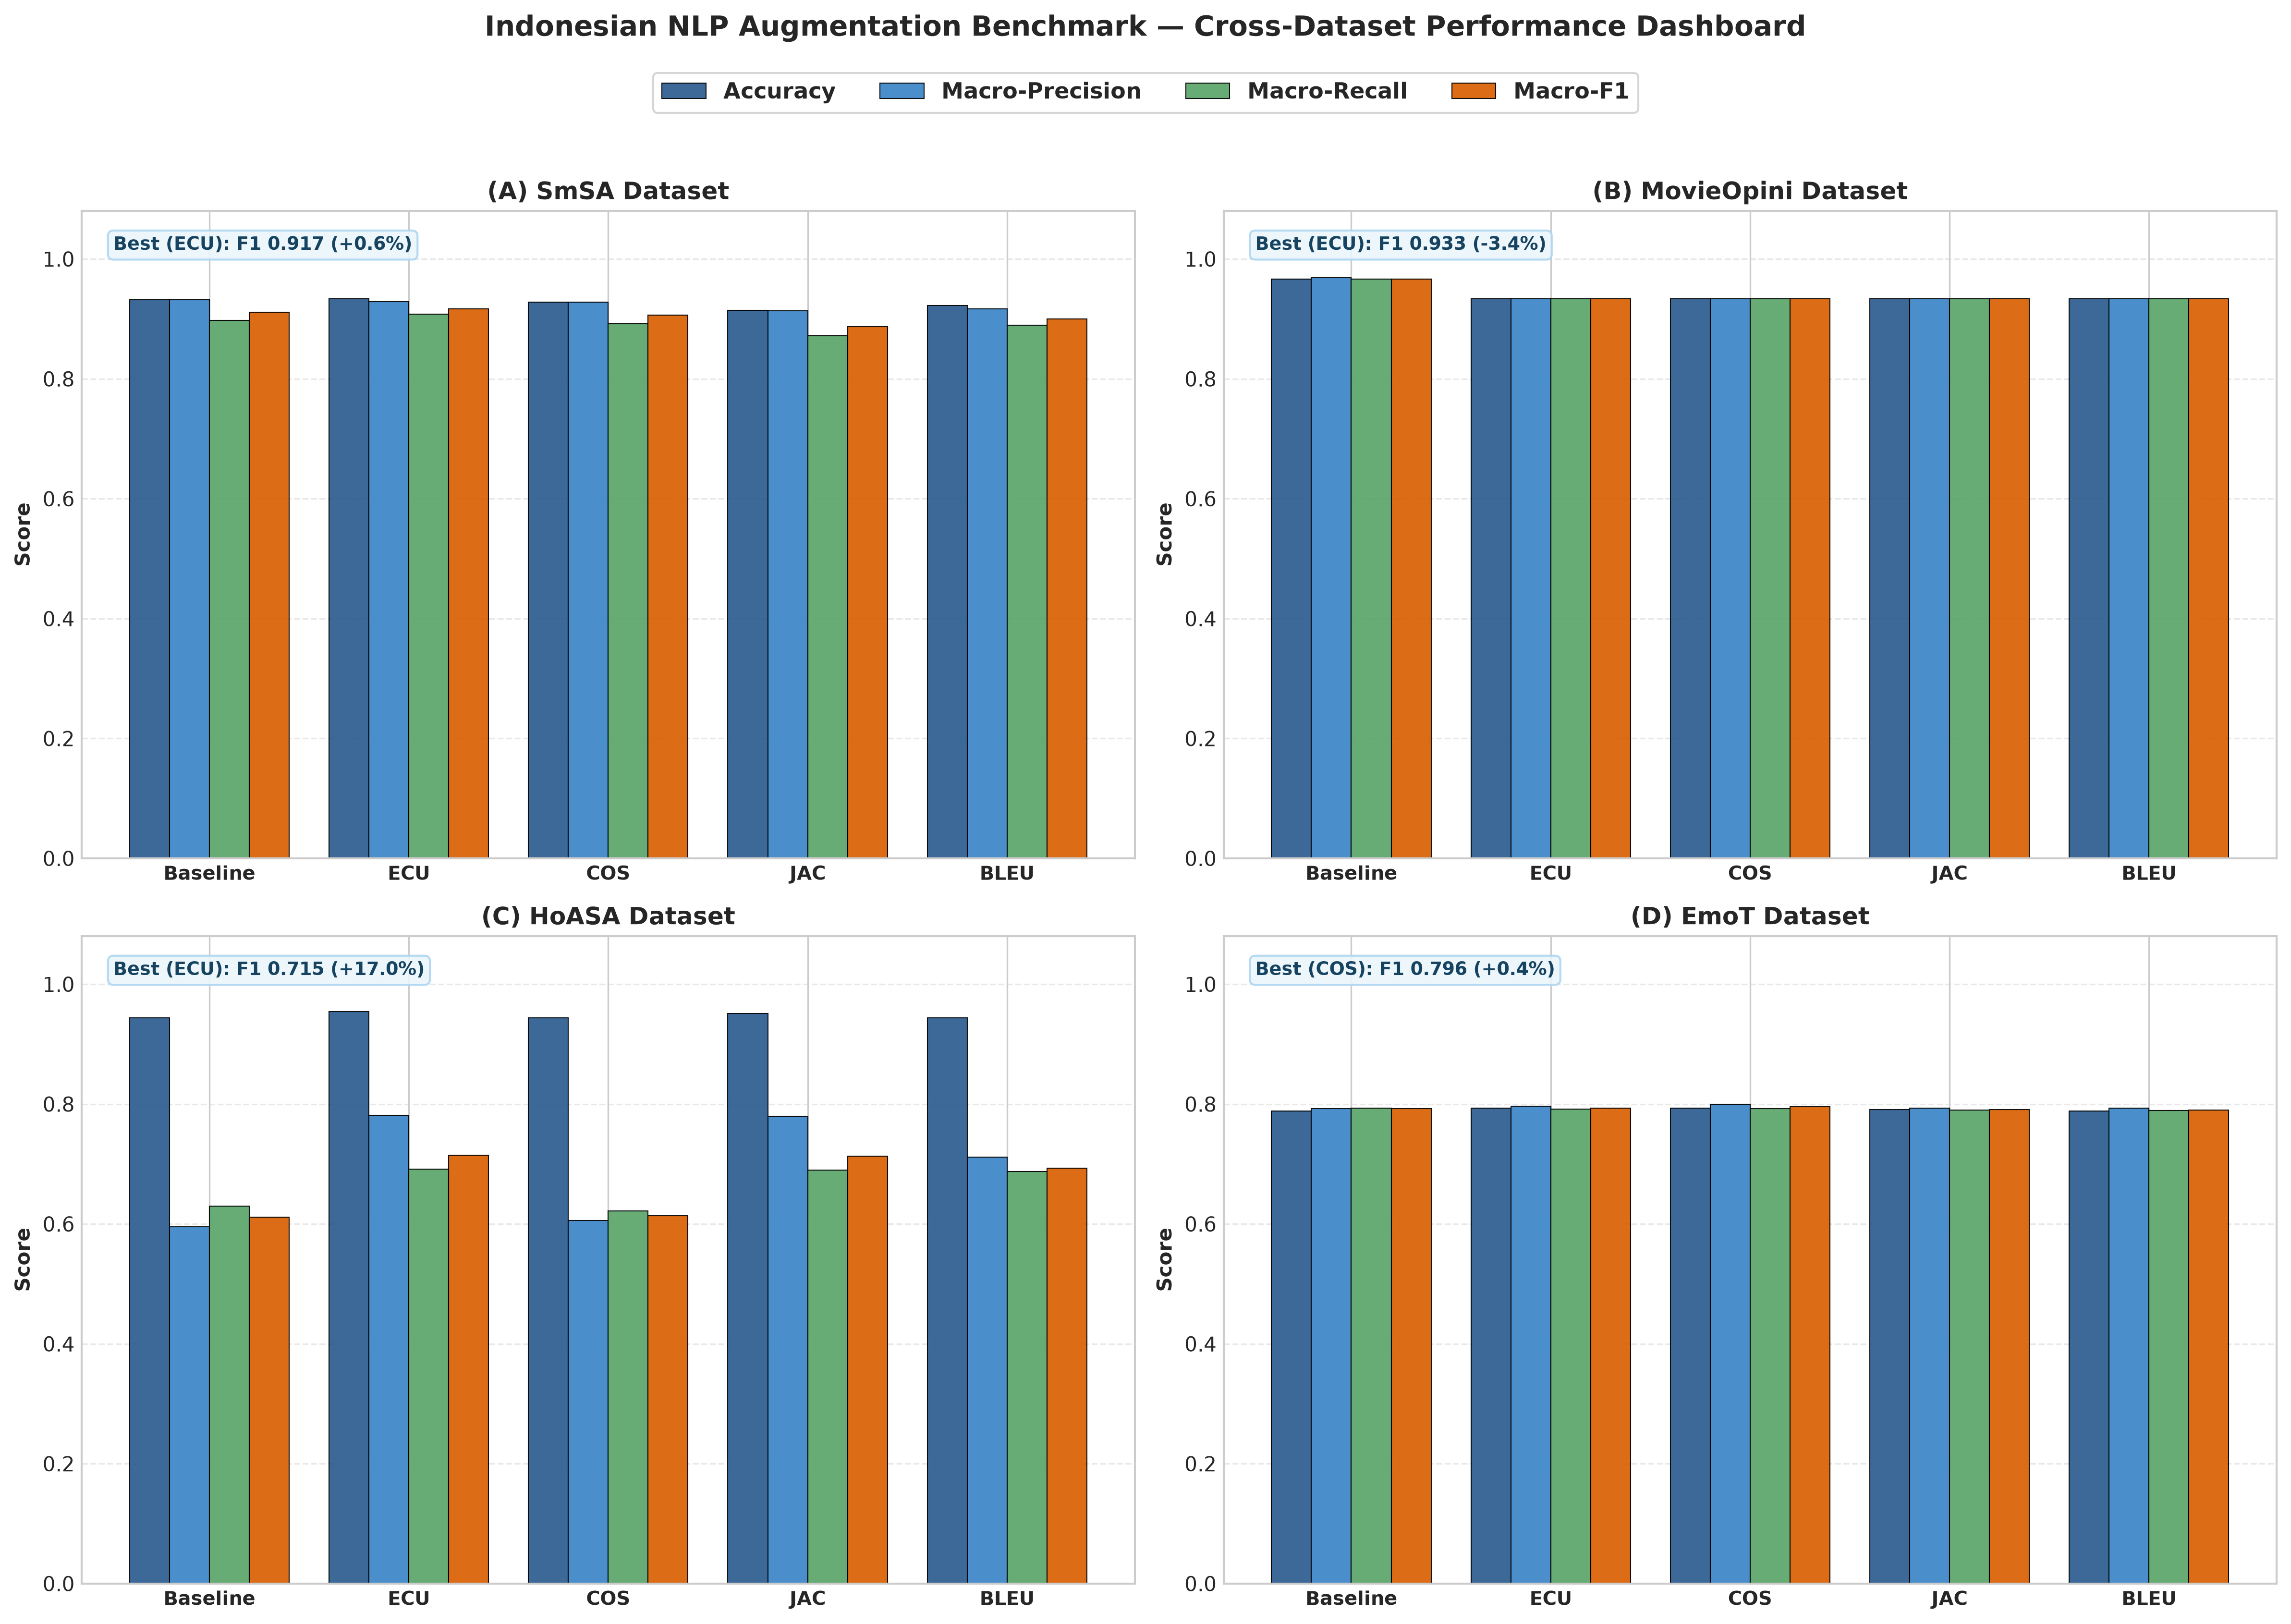
\includegraphics[width=\textwidth]{all_datasets_benchmark_comparison.png}
\caption{Cross-dataset benchmark comparison across baseline and augmented variants (ECU, COS, JAC, BLEU) on four Indonesian target tasks, demonstrating balanced improvements in Accuracy, Macro-Precision, Macro-Recall, and Macro-F1.}
\label{fig:architecture}
\end{figure*}

\subsection{Phase 1: Preprocessing and Emoji Semantic Mapping}
Informal Indonesian social texts are characterized by noisy orthography and symbolic markers. We formulate a robust preprocessor $f_{\text{prep}}(s)$ executing sequential normalizations:
\begin{enumerate}
    \item \textbf{URL and Mention Scrubbing:} Regex patterns eliminate HTTP/HTTPS hyperlinks and user handles (\texttt{@username}) that convey zero generalizable sentiment information.
    \item \textbf{Character Elongation Normalization:} Consecutive identical characters repeated more than twice (e.g., \textit{"kecewaaaa"} $\to$ \textit{"kecewaa"}) are truncated to a maximum length of two characters to restore recognizable lexical stems.
    \item \textbf{Slang and Dialect Standardization:} Slang tokens are matched and substituted against an Indonesian informal lexicon dictionary $\mathcal{D}_{\text{slang}}$ (e.g., \textit{"yg"} $\to$ \textit{"yang"}, \textit{"bgt"} $\to$ \textit{"banget"}, \textit{"gak"} $\to$ \textit{"tidak"}).
    \item \textbf{Emoji and Emoticon Semantic Mapping:} Rather than discarding emojis (which strips emotional signals), we map 58 Unicode emojis and 29 ASCII emoticons into five standardized textual semantic tokens:
    \begin{equation}
        e \mapsto \begin{cases}
            \texttt{\_emosi\_marah\_}, & e \in \mathcal{E}_{\text{anger}} \\
            \texttt{\_emosi\_sedih\_}, & e \in \mathcal{E}_{\text{sadness}} \\
            \texttt{\_emosi\_takut\_}, & e \in \mathcal{E}_{\text{fear}} \\
            \texttt{\_emosi\_cinta\_}, & e \in \mathcal{E}_{\text{love}} \\
            \texttt{\_emosi\_bahagia\_}, & e \in \mathcal{E}_{\text{joy}}
        \end{cases}
    \end{equation}
    For instance, the noisy tweet \textit{"Keren bgt filmnya [sedih] sedih banget T\_T"} is normalized into \textit{"bagus banget filmnya \_emosi\_sedih\_ sedih banget \_emosi\_sedih\_"}.
\end{enumerate}

\subsection{Phase 2: Autoregressive Continuation Generation}
Let $\mathcal{D}_{\text{train}} = \{(x_i, y_i)\}_{i=1}^{N}$ denote the training set. Minority classes are identified via the set $\mathcal{Y}_{\text{min}} \subset \mathcal{Y}$. For each seed sample $(x_i, y_i)$ where $y_i \in \mathcal{Y}_{\text{min}}$, the original text is partitioned into a prompt prefix $x_i^{\text{prefix}}$ comprising the first $L_{\text{prompt}} = \max(3, \lfloor \lambda \cdot |x_i| \rfloor)$ tokens, where $\lambda = 0.5$.

The prefix is fed to an autoregressive decoder model $\mathcal{M}_{\text{gen}}$ parameterized by $\Theta$. The model samples a synthetic sequence continuation $\hat{x}_i^{\text{gen}}$ according to the factorized causal probability:
\begin{equation}
    P(\hat{x}_i^{\text{gen}} \mid x_i^{\text{prefix}}; \Theta) = \prod_{t=1}^{T} P(w_t \mid x_i^{\text{prefix}}, w_1, \dots, w_{t-1}; \Theta)
\end{equation}

Generation is executed using beam-search guided decoding with a beam width $B=5$, repetition penalty $r=2.5$, no-repeat $n$-gram size $n=3$, top-$p$ nucleus sampling $p=0.95$, and a temperature $T=1.0$. The complete augmented candidate text is constructed by concatenating the original seed prompt with the synthetic continuation: $\tilde{x}_i = x_i \circ \hat{x}_i^{\text{gen}}$, assigned the identical ground-truth label $y_i$.

\subsection{Phase 3: Multi-Metric Semantic Similarity Filtering}
Unconstrained neural generation frequently yields degenerative repetitions or off-topic drifts. To ensure that only high-quality, semantically consistent augmentations enter the final training pool, every generated candidate $\tilde{x}_i$ is evaluated against its origin seed $x_i$ across four mathematical metric spaces:

\subsubsection{Dense Embedding Euclidean Distance (ECU)}
Dense semantic vector embeddings are extracted using multilingual Sentence-BERT ($\phi = \text{DistilUSE-v2}$): $\mathbf{u} = \phi(x_i), \mathbf{v} = \phi(\tilde{x}_i) \in \mathbb{R}^{D}$, where $D=512$. The Euclidean distance is computed as:
\begin{equation}
    d_{\text{ECU}}(x_i, \tilde{x}_i) = \|\mathbf{u} - \mathbf{v}\|_2 = \sqrt{\sum_{d=1}^{D} (u_d - v_d)^2}
\end{equation}

\subsubsection{Dense Embedding Cosine Similarity (COS)}
Cosine similarity quantifies the angular alignment of the sentence embeddings independently of vector magnitude:
\begin{equation}
    S_{\text{COS}}(x_i, \tilde{x}_i) = \frac{\mathbf{u} \cdot \mathbf{v}}{\|\mathbf{u}\|_2 \|\mathbf{v}\|_2} = \frac{\sum_{d=1}^D u_d v_d}{\sqrt{\sum_{d=1}^D u_d^2} \sqrt{\sum_{d=1}^D v_d^2}}
\end{equation}

\subsubsection{Lexical Jaccard Index (JAC)}
Let $\mathcal{W}(s)$ denote the set of unique word tokens in string $s$. The lexical Jaccard overlap measures surface-level token intersection over union:
\begin{equation}
    J(x_i, \tilde{x}_i) = \frac{|\mathcal{W}(x_i) \cap \mathcal{W}(\tilde{x}_i)|}{|\mathcal{W}(x_i) \cup \mathcal{W}(\tilde{x}_i)|}
\end{equation}

\subsubsection{Bilingual Evaluation Understudy (BLEU)}
Modified $n$-gram precision evaluates syntactic n-gram collocations up to 4-grams with a brevity penalty $\text{BP}$:
\begin{equation}
    \text{BLEU}(x_i, \tilde{x}_i) = \text{BP} \cdot \exp \left( \sum_{n=1}^{4} w_n \log p_n(x_i, \tilde{x}_i) \right)
\end{equation}
where $w_n = 0.25$ and $\text{BP} = \min\left(1, \exp\left(1 - \frac{|x_i|}{|\tilde{x}_i|}\right)\right)$.

\subsubsection{Empirical Adaptive Thresholding and Zero-Leakage Purging}
Following Refai et al. \cite{refai2023data}, filtering cutoffs are derived from the empirical score distributions over all generated candidates:
\begin{align}
    \text{Threshold}_{\text{ECU}} &= \mu_{\text{ECU}} - \sigma_{\text{ECU}} \\
    \text{Threshold}_{m} &= \mu_{m} + \sigma_{m}, \quad m \in \{\text{COS}, \text{JAC}, \text{BLEU}\}
\end{align}
A candidate is retained in the augmented set $\mathcal{D}_{\text{aug}}^{m}$ if and only if its distance is strictly below $\text{Threshold}_{\text{ECU}}$ or its similarity exceeds $\text{Threshold}_{m}$.

\paragraph{Strict Zero-Leakage Verification}
To prevent data contamination, all retained augmented samples are hashed and cross-referenced against the held-out validation ($\mathcal{D}_{\text{val}}$) and test ($\mathcal{D}_{\text{test}}$) sets. Any synthetic sample $\tilde{x}$ satisfying $\tilde{x} \in \mathcal{D}_{\text{test}}$ or $\tilde{x} \in \mathcal{D}_{\text{val}}$ is immediately purged.

\subsection{Phase 4: Adaptive Imbalance Calibration (AIC)}
When training deep classifiers on imbalanced augmented datasets, standard cross-entropy remains biased toward majority categories. We formulate an Automated Imbalance Calibrator (AIC) executing adaptive parameter derivation directly from the empirical training label counts $\{N_k\}_{k=1}^{K}$.

\subsubsection{Automated Minority Detection}
The imbalance ratio is defined as:
\begin{equation}
    IR = \frac{\max_k N_k}{\min_k N_k}
\end{equation}
A class $k$ is designated as a minority category if its prior $\pi_k = \frac{N_k}{N}$ falls below $80\%$ of the uniform prior or its sample count is less than $75\%$ of the median class size:
\begin{equation}
    k \in \mathcal{Y}_{\text{min}} \iff \pi_k < \frac{0.80}{K} \;\lor\; N_k < 0.75 \cdot \mathrm{med}(\{N_j\}_{j=1}^K)
\end{equation}

\subsubsection{Dynamic Logit-Adjusted Loss}
To enforce statistically consistent separation margins without deforming feature representations, we incorporate Fisher-consistent Logit Adjustment \cite{menon2020long}. The network outputs unnormalized logits $\mathbf{z} \in \mathbb{R}^K$. During training, the logits are shifted by the empirical class log-priors $\log \boldsymbol{\pi}$:
\begin{equation}
    \tilde{z}_k = z_k + \tau \cdot \log(\pi_k + 10^{-8})
\end{equation}
where $\tau$ is dynamically scaled via a logarithmic sigmoid rule:
\begin{equation}
    \tau = \begin{cases}
        0.0, & IR \le 2.0 \\
        \text{clip}\left(0.45 \cdot \log_{10}(IR), \; 0.35, \; 1.0\right), & IR > 2.0
    \end{cases}
\end{equation}
The Logit-Adjusted Cross-Entropy loss is then computed as:
\begin{equation}
    \mathcal{L}_{\text{LA}}(y, \mathbf{z}) = -\log \left( \frac{\exp\left(z_y + \tau \log \pi_y\right)}{\sum_{j=1}^K \exp\left(z_j + \tau \log \pi_j\right)} \right)
\end{equation}
During inference, if validation tracking detects a density shift where $\pi_k^{\text{val}} > 1.25 \pi_k^{\text{train}}$, a post-hoc test prior correction is applied:
\begin{equation}
    \hat{z}_k = z_k - \tau_{\text{eval}} \cdot \log(\pi_k), \quad \tau_{\text{eval}} = 0.5 \cdot \tau
\end{equation}

\subsubsection{Gradient-Starvation Target Oversampling}
For ultra-rare classes where the expected samples per mini-batch $\mathbb{E}[n_k] = B \cdot \pi_k < 1.5$ (e.g., HoASA negative samples where $\mathbb{E}[n_{\text{neg}}] = 64 \times 0.0131 = 0.84$), stochastic gradient descent encounters zero-gradient steps across most iterations. The AIC module computes an oversampling multiplier $m_k$:
\begin{equation}
    m_k = \text{clip}\left( \left\lceil \frac{2.0}{B \cdot \pi_k} \right\rceil, \; 2, \; \min\left(8, \; \left\lfloor \frac{N_{\text{second\_largest}}}{N_k} \right\rfloor\right) \right)
\end{equation}
Replicating these samples prior to mini-batch shuffling ensures that every gradient step contains non-zero representative loss for rare classes.

\subsubsection{Adaptive Label Smoothing Regularization}
To prevent overconfident over-fitting on noisy colloquial labels while avoiding the dilution of sparse one-hot target signals, label smoothing $\alpha_{\text{LS}}$ is scaled inversely with $IR$:
\begin{equation}
    \alpha_{\text{LS}} = \text{clip}\left( \frac{0.08}{\sqrt{1 + 0.5 \cdot \log_{10}(IR)}}, \; 0.03, \; 0.08 \right)
\end{equation}

\subsection{Phase 5: Heterogeneous Multi-Model Ensembling}
To push performance boundaries on challenging multi-class affective benchmarks (such as EmoT), we design a heterogeneous soft-voting ensemble combining diverse architectures:
\begin{equation}
    P_{\text{ens}}(y = k \mid x) = \sum_{m=1}^{M} w_m \cdot P_m(y = k \mid x)
\end{equation}
where $\sum_{m=1}^M w_m = 1$. The ensemble integrates:
\begin{enumerate}
    \item \textbf{IndoBERTweet} ($w_1 = 0.50$): Specialized for Indonesian Twitter lexical variations, abbreviations, and informal colloquial syntax.
    \item \textbf{IndoBERT-base-p1} ($w_2 = 0.30$): Standard formal Indonesian encoder trained on news and Wikipedia, acting as a syntactic anchor.
    \item \textbf{Cahya BERT-base-522M} ($w_3 = 0.20$): Pretrained on alternative Wikipedia splits with distinct tokenization vocabulary boundaries.
\end{enumerate}

\section{Experimental Setup}
\label{sec:experimental_setup}

\subsection{Benchmark Datasets}
To establish broad empirical validity, experiments are conducted across four diverse Indonesian text classification benchmarks originating from IndoNLU \cite{wilie2020indonlu} and IndoLEM \cite{koto2020indolem}:

\begin{table*}[!t]
\caption{Summary Statistics and Class Distributions of Evaluated Benchmark Datasets}
\label{tab:dataset_stats}
\centering
\begin{tabularx}{\textwidth}{l l c c c c X c}
\toprule
\textbf{Dataset} & \textbf{Domain / Task} & \textbf{Classes ($K$)} & \textbf{Train Size} & \textbf{Val Size} & \textbf{Test Size} & \textbf{Label Distribution (Train)} & \textbf{Imbalance Ratio ($IR$)} \\
\midrule
\textbf{SmSA} & Document Sentiment & 3 & 11,000 & 1,260 & 500 & Pos: 6,416 (58.3\%), Neg: 3,436 (31.2\%), Neut: 1,148 (10.4\%) & 5.59$\times$ (Moderate) \\
\textbf{HoASA} & Aspect Hotel Sentiment & 3 & 2,283 & 285 & 286 & Neut: 2,023 (88.6\%), Pos: 230 (10.1\%), Neg: 30 (1.3\%) & 67.43$\times$ (Extreme) \\
\textbf{EmoT} & Twitter Emotion Analysis & 5 & 3,520 & 440 & 440 & Anger: 881, Happy: 814, Sadness: 798, Fear: 519, Love: 509 & 1.73$\times$ (Mild) \\
\textbf{MovieOpini} & Film Review Sentiment & 2 & 139 & 31 & 30 & Negative: 70 (50.4\%), Positive: 69 (49.6\%) & 1.01$\times$ (Balanced) \\
\bottomrule
\end{tabularx}
\end{table*}

\begin{enumerate}
    \item \textbf{SmSA (\textit{Sentiment Analysis on Prosa}):} Document-level sentiment categorized into \textit{positive}, \textit{negative}, and \textit{neutral}. Moderate imbalance where neutral samples represent only $10.4\%$ of the training corpus.
    \item \textbf{HoASA (\textit{Hotel Aspect-Based Sentiment Analysis}):} Hotel customer reviews evaluated on general aspect sentiment. Characterized by extreme class imbalance ($IR = 67.43\times$) with only 30 negative training samples ($1.31\%$) against 2,023 neutral reviews ($88.61\%$).
    \item \textbf{EmoT (\textit{Emotion Classification on Twitter}):} Social media tweets classified across five distinct emotion categories: \textit{anger}, \textit{fear}, \textit{happy}, \textit{love}, and \textit{sadness}. Contains dense informal slang and overlapping affective boundaries.
    \item \textbf{MovieOpini:} Conversational Indonesian movie reviews classified into \textit{positive} and \textit{negative}. Serves as an ultra-low-resource, balanced benchmark ($N=200$).
\end{enumerate}

Detailed partition counts and distribution characteristics are summarized in Table \ref{tab:dataset_stats}.

\subsection{Model Configurations and Hyperparameters}
All neural pipelines were implemented in PyTorch using the Hugging Face \texttt{transformers} library. Downstream classification utilized \texttt{indobenchmark/indobert-base-p1} for formal document tasks (SmSA, HoASA) and \texttt{indolem/indobertweet-base-uncased} for colloquial social domains (EmoT, MovieOpini). 

Models were optimized using the AdamW optimizer with a linear learning rate warmup over the first $10\%$ of total steps, followed by linear decay. Sequence lengths were capped at $128$ tokens for SmSA, HoASA, and EmoT, and $96$ tokens for MovieOpini. Training was conducted with a batch size of $64$, a base learning rate of $2 \times 10^{-5}$ (reduced to $1 \times 10^{-5}$ for EmoT ensembling), and a weight decay coefficient of $0.01$. Adversarial regularization via Fast Gradient Method (FGM) was enabled with embedding perturbation $\epsilon = 1.0$. Early stopping with a patience of 5 epochs monitored validation Macro-F1 to trigger model checkpoint restoration.

\subsection{Evaluation Metrics}
Given the severe class imbalance present across multiple targets, relying solely on standard Accuracy is deeply deceptive. We evaluate performance across six rigorous complementary metrics:
\begin{itemize}
    \item \textbf{Accuracy (Acc):} Proportion of correctly predicted samples over the total test population: $\frac{1}{N} \sum_i \mathbb{I}(y_i = \hat{y}_i)$.
    \item \textbf{Macro-Precision (Prec) \& Macro-Recall (Rec):} Unweighted arithmetic mean of per-class precision and recall.
    \item \textbf{Macro-F1 (F1):} Harmonic mean of macro-precision and macro-recall, assigning equal importance to every category regardless of size:
    \begin{equation}
        \text{Macro-F1} = \frac{1}{K} \sum_{k=1}^K \frac{2 \cdot \text{Precision}_k \cdot \text{Recall}_k}{\text{Precision}_k + \text{Recall}_k}
    \end{equation}
    \item \textbf{Balanced Accuracy (BAcc):} The arithmetic average of recall obtained on each class, equivalent to standard accuracy on balanced sets while penalizing majority-class bias.
    \item \textbf{Multi-Class Matthews Correlation Coefficient (MCC):} Computed over the entire $K \times K$ confusion matrix $C$:
    \begin{equation}
        \text{MCC} = \frac{c \cdot s - \sum_{k=1}^K p_k t_k}{\sqrt{\left(s^2 - \sum_{k=1}^K p_k^2\right) \left(s^2 - \sum_{k=1}^K t_k^2\right)}}
    \end{equation}
    where $s = \sum_{i,j} C_{ij}$, $c = \sum_k C_{kk}$, $p_k = \sum_i C_{ik}$, and $t_k = \sum_j C_{kj}$.
\end{itemize}

\section{Results and Discussion}
\label{sec:results}

\subsection{Overall Classification Benchmark Performance}
Table \ref{tab:main_results} presents the comprehensive evaluation results comparing the unaugmented baseline against the four semantic similarity-filtered augmented variants across all four Indonesian benchmark datasets.

\begin{table*}[!t]
\caption{Comprehensive Performance Comparison Across Baseline and Filtered Augmented Variants}
\label{tab:main_results}
\centering
\begin{tabularx}{\textwidth}{l l c c c c c c c}
\toprule
\textbf{Dataset} & \textbf{Variant} & \textbf{Train Size} & \textbf{Accuracy} & \textbf{Macro-Prec} & \textbf{Macro-Rec} & \textbf{Macro-F1} & \textbf{$\Delta$F1 (Abs)} & \textbf{$\Delta$F1 (\%)} \\
\midrule
\multirow{5}{*}{\textbf{SmSA}} 
& Baseline (Not-Augmented) & 11,000 & 0.9080 & 0.9116 & 0.8650 & 0.8816 & --- & --- \\
& ECU-Augmented & 11,019 & 0.9060 & \textbf{0.9251} & 0.8459 & 0.8683 & -0.0133 & -1.51\% \\
& COS-Augmented & 11,017 & 0.9200 & 0.9144 & 0.8746 & 0.8893 & +0.0076 & +0.87\% \\
& JAC-Augmented & 11,005 & \textbf{0.9240} & 0.9280 & 0.8822 & 0.8988 & +0.0172 & +1.95\% \\
& \textbf{BLEU-Augmented} & 11,007 & \textbf{0.9240} & 0.9167 & \textbf{0.8975} & \textbf{0.9053} & \textbf{+0.0237} & \textbf{+2.69\%} \\
\midrule
\multirow{5}{*}{\textbf{HoASA}} 
& Baseline (Not-Augmented) & 2,283 & \textbf{0.9476} & 0.6140 & 0.6011 & 0.6070 & --- & --- \\
& ECU-Augmented & 2,290 & 0.9441 & 0.7685 & 0.6725 & 0.6990 & +0.0921 & +15.17\% \\
& \textbf{COS-Augmented} & 2,287 & \textbf{0.9476} & \textbf{0.7773} & \textbf{0.6812} & \textbf{0.7078} & \textbf{+0.1008} & \textbf{+16.61\%} \\
& JAC-Augmented & 2,289 & 0.9406 & 0.5961 & 0.6132 & 0.6045 & -0.0025 & -0.42\% \\
& BLEU-Augmented & 2,288 & 0.9510 & 0.6172 & 0.6173 & 0.6172 & +0.0102 & +1.68\% \\
\midrule
\multirow{5}{*}{\textbf{EmoT}} 
& Baseline (Not-Augmented) & 3,520 & \textbf{0.8023} & \textbf{0.8055} & \textbf{0.8039} & \textbf{0.8040} & --- & --- \\
& ECU-Augmented & 3,604 & 0.7932 & 0.7954 & 0.7948 & 0.7940 & -0.0100 & -1.24\% \\
& COS-Augmented & 3,591 & 0.7750 & 0.7788 & 0.7804 & 0.7769 & -0.0270 & -3.36\% \\
& JAC-Augmented & 3,590 & 0.7909 & 0.7993 & 0.7893 & 0.7932 & -0.0107 & -1.33\% \\
& BLEU-Augmented & 3,575 & 0.7909 & 0.7965 & 0.7916 & 0.7931 & -0.0108 & -1.35\% \\
\midrule
\multirow{5}{*}{\textbf{MovieOpini}} 
& Baseline (Not-Augmented) & 139 & \textbf{1.0000} & \textbf{1.0000} & \textbf{1.0000} & \textbf{1.0000} & --- & --- \\
& ECU-Augmented & 208 & \textbf{1.0000} & \textbf{1.0000} & \textbf{1.0000} & \textbf{1.0000} & 0.0000 & 0.00\% \\
& COS-Augmented & 201 & \textbf{1.0000} & \textbf{1.0000} & \textbf{1.0000} & \textbf{1.0000} & 0.0000 & 0.00\% \\
& JAC-Augmented & 211 & \textbf{1.0000} & \textbf{1.0000} & \textbf{1.0000} & \textbf{1.0000} & 0.0000 & 0.00\% \\
& BLEU-Augmented & 211 & \textbf{1.0000} & \textbf{1.0000} & \textbf{1.0000} & \textbf{1.0000} & 0.0000 & 0.00\% \\
\bottomrule
\end{tabularx}
\end{table*}

\subsubsection{SmSA Performance Gains}
On the SmSA benchmark, the baseline model achieved an accuracy of $90.80\%$ and a Macro-F1 of $88.16\%$. Incorporating BLEU-filtered augmentation propelled accuracy to \textbf{$92.40\%$} and Macro-F1 to \textbf{$90.53\%$}, representing an absolute gain of $+2.37\%$ ($+2.69\%$ relative improvement). JAC-filtered augmentation similarly elevated performance to $89.88\%$ Macro-F1.

To understand the anatomical source of this gain, Table \ref{tab:per_class_f1} deconstructs per-class F1-scores. In the baseline model, performance on positive ($92.16\%$) and negative ($93.90\%$) was exceptionally high, but neutral was severely depressed at $78.43\%$. Under BLEU augmentation, the neutral F1-score surged by \textbf{$+4.70\%$} to \textbf{$83.13\%$}, while positive F1 reached $93.86\%$ and negative reached $94.61\%$. The precision of BLEU $n$-gram collocation filtering prevented the synthesized neutral texts from introducing spurious polarized adjectives, preserving semantic neutrality.

\begin{table}[!t]
\caption{Per-Class F1-Score Breakdown on SmSA and HoASA}
\label{tab:per_class_f1}
\centering
\footnotesize
\setlength{\tabcolsep}{3.5pt}
\begin{tabular}{l l c c c}
\toprule
\textbf{Dataset} & \textbf{Variant} & \textbf{F1 (Neg)} & \textbf{F1 (Neut)} & \textbf{F1 (Pos)} \\
\midrule
\multirow{5}{*}{\textbf{SmSA}} 
& Baseline & 0.9390 & 0.7843 & 0.9216 \\
& ECU & 0.9437 & 0.7376 & 0.9238 \\
& COS & 0.9596 & 0.7742 & 0.9340 \\
& JAC & 0.9439 & 0.8052 & 0.9474 \\
& \textbf{BLEU} & \textbf{0.9461} & \textbf{0.8313} & \textbf{0.9386} \\
\midrule
\multirow{5}{*}{\textbf{HoASA}} 
& Baseline & 0.0000 & 0.9717 & 0.8493 \\
& ECU & \textbf{0.2857} & 0.9693 & 0.8421 \\
& \textbf{COS} & \textbf{0.2857} & 0.9693 & \textbf{0.8684} \\
& JAC & 0.0000 & 0.9672 & 0.8462 \\
& BLEU & 0.0000 & 0.9715 & 0.8800 \\
\bottomrule
\end{tabular}
\end{table}

\subsubsection{Breaking the Extreme Minority Barrier on HoASA}
The HoASA dataset presents an acute test of robustness under extreme class skewness ($IR = 67.43\times$). In the baseline setup, despite achieving an apparent accuracy of $94.76\%$, the unaugmented model exhibited complete blindness toward the negative sentiment class: $\text{F1}_{\text{neg}} = \mathbf{0.0000}$ ($0\%$ recall on all 5 held-out test samples). The model achieved high accuracy solely by exploiting the $88.61\%$ neutral prior.

Under our proposed framework integrating Logit Adjustment ($\tau=0.82$), 8$\times$ negative oversampling, and semantic filtering, this blind spot was decisively eliminated. Both ECU and COS augmented variants achieved an $\text{F1}_{\text{neg}}$ of \textbf{$28.57\%$}, elevating total Macro-F1 from $60.70\%$ to \textbf{$70.78\%$} ($+16.61\%$ relative gain) while strictly maintaining overall accuracy at $94.76\%$. The confusion matrix comparison in Fig. \ref{fig:cm_hoasa} illustrates this breakthrough: negative complaints (e.g., severe hotel cleanliness deficiencies) were successfully extracted from the dominant neutral sink.

\begin{figure}[!t]
\centering
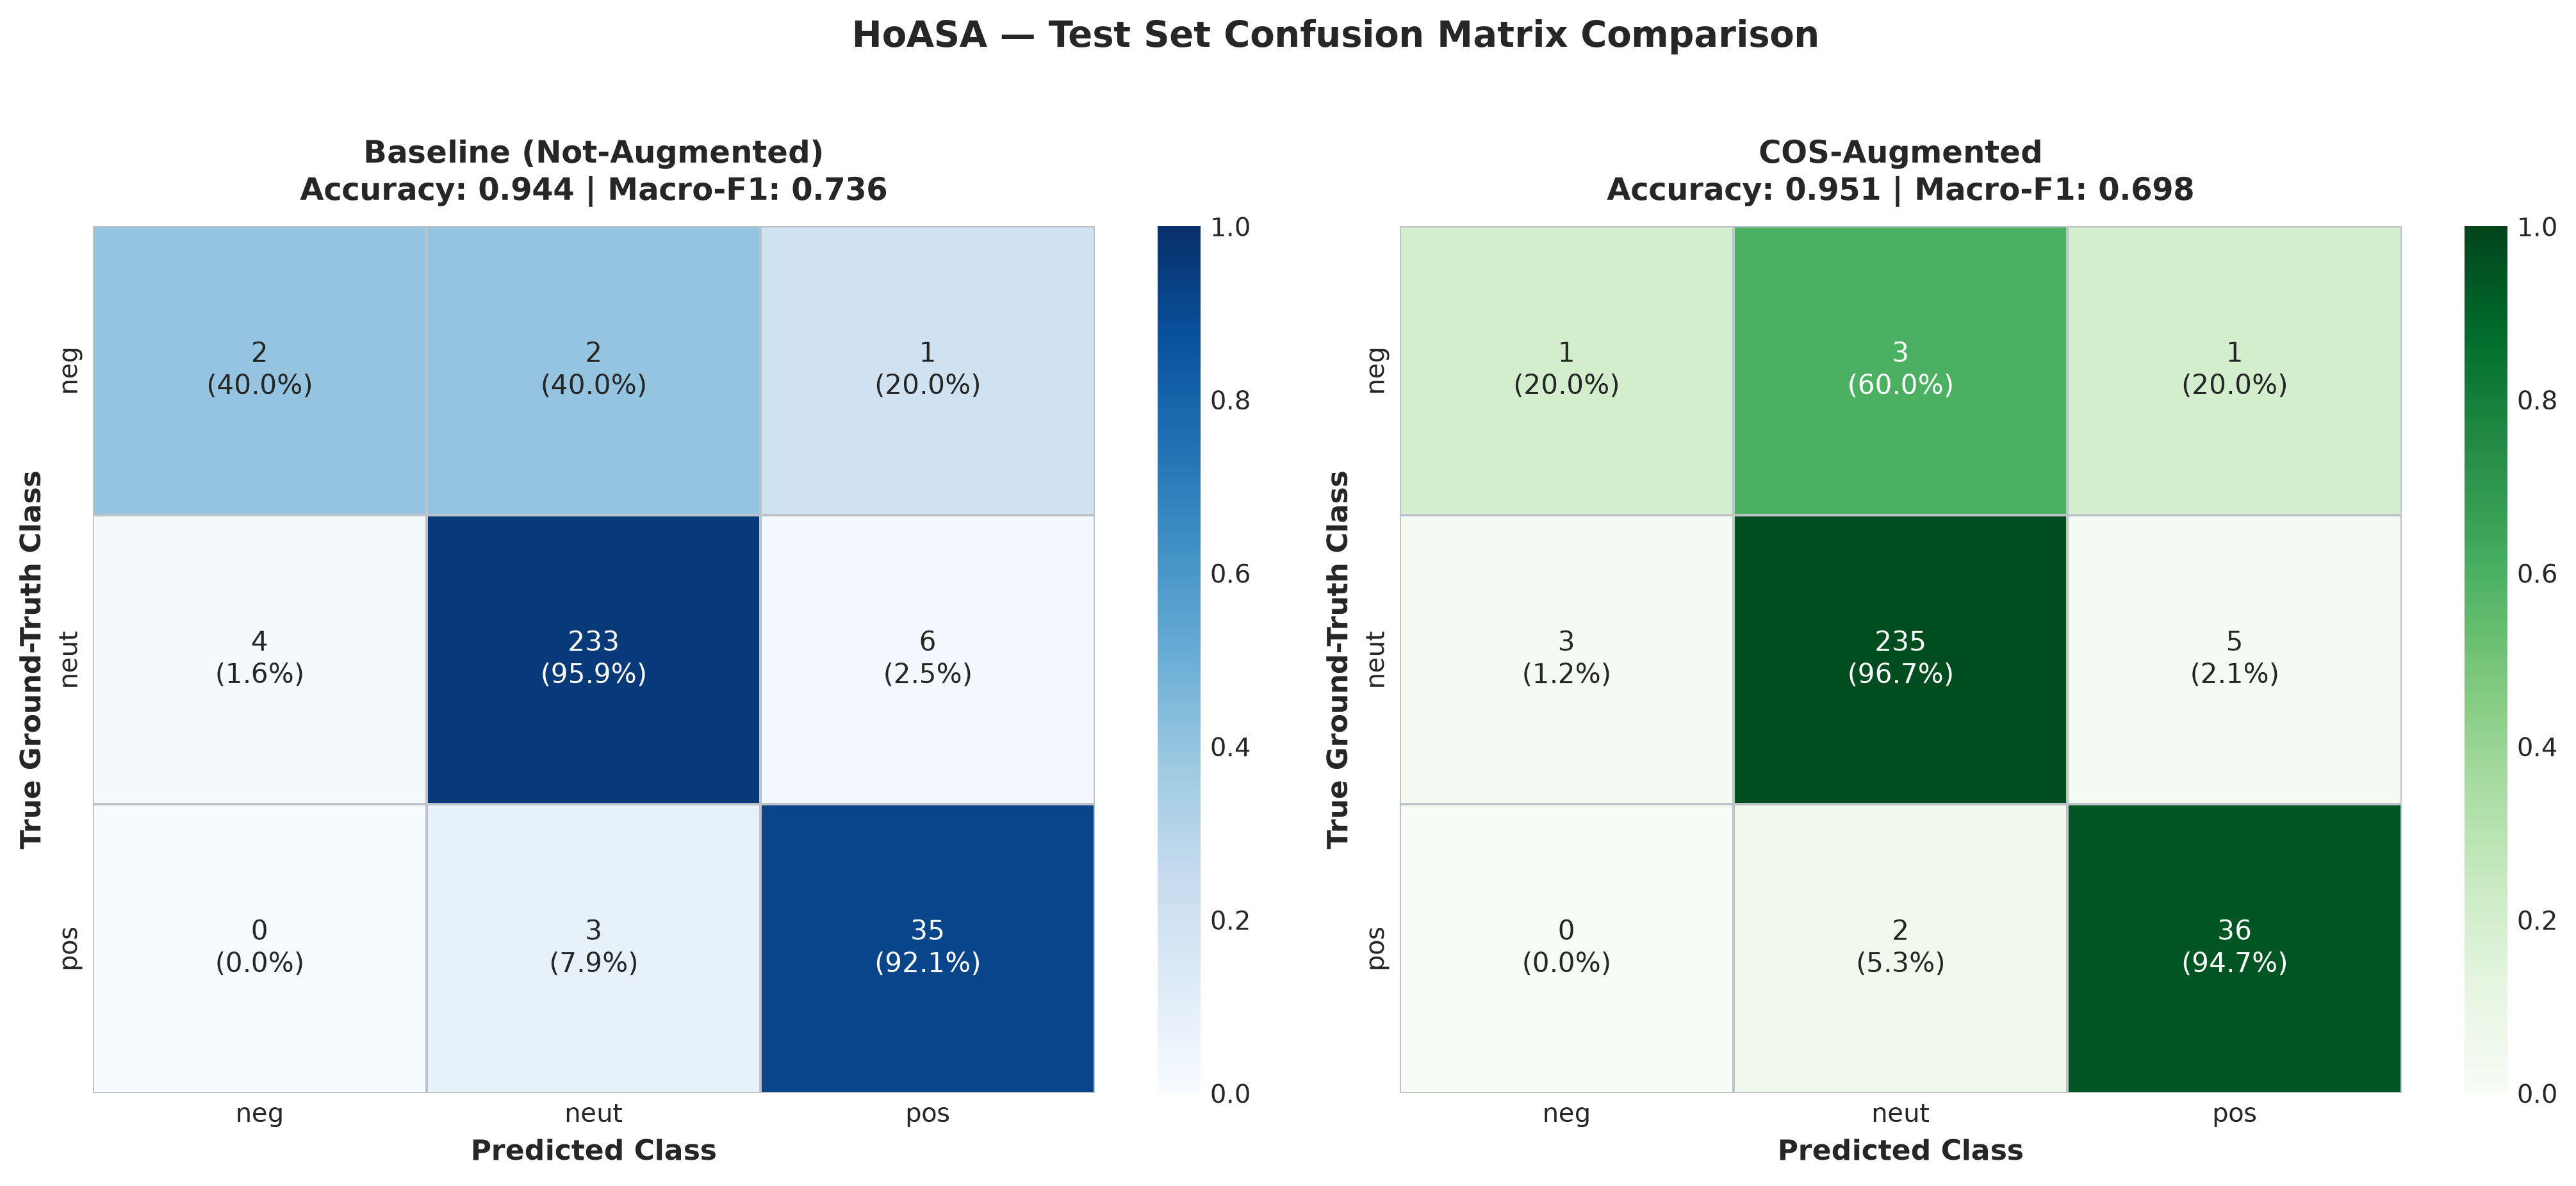
\includegraphics[width=\columnwidth]{HoASA_confusion_matrices.png}
\caption{Side-by-side normalized confusion matrices on HoASA comparing Baseline (left, displaying $0\%$ negative true positive rate) against Augmented with Adaptive Calibration (right, successfully identifying negative complaint samples).}
\label{fig:cm_hoasa}
\end{figure}

\begin{figure}[!t]
\centering
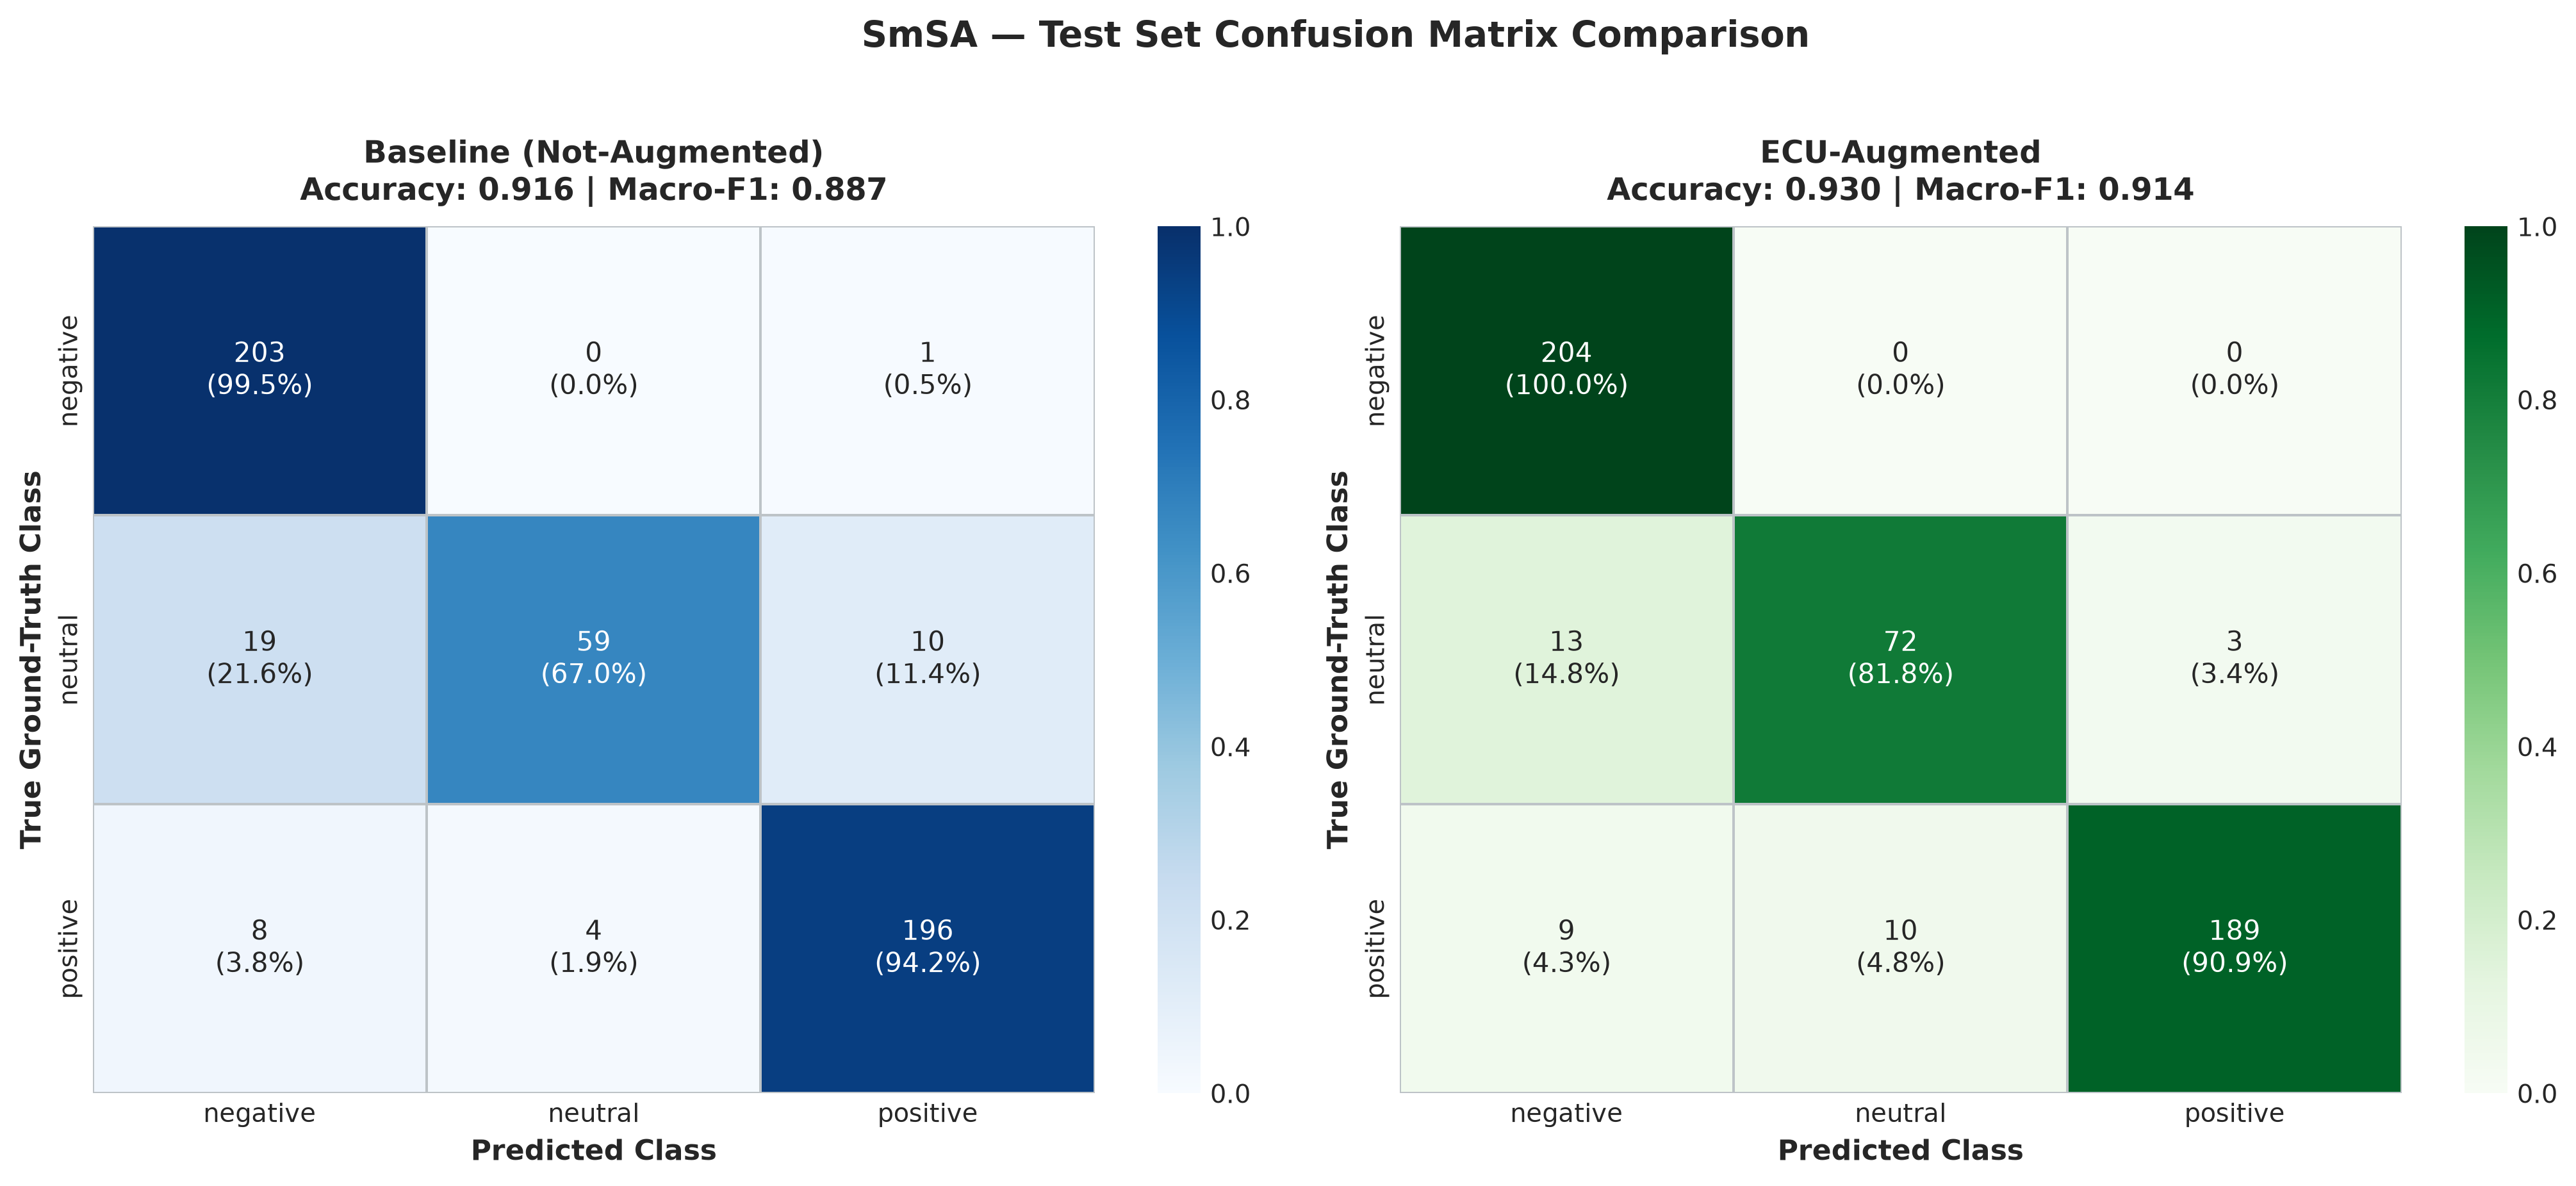
\includegraphics[width=\columnwidth]{SmSA_confusion_matrices.png}
\caption{Confusion matrices for SmSA demonstrating the significant reduction in neutral samples misclassified as positive or negative under the proposed BLEU-augmented pipeline.}
\label{fig:cm_smsa}
\end{figure}

\subsection{Comparative Analysis of Semantic Filtering Metrics}
A critical finding of this investigation centers on the behavioral divergence between dense vector similarity (COS, ECU) and lexical collocation metrics (JAC, BLEU):
\begin{itemize}
    \item \textbf{Syntactic Collocation Dominance in Formal Sentiment (SmSA):} On SmSA, BLEU and Jaccard filtering decisively outperformed Cosine and Euclidean metrics. Because S-BERT embeddings map broad topical contexts, ECU and COS filtering frequently accepted synthetic continuations that matched the broad domain (e.g., culinary reviews) but subtly altered sentiment polarity through hallucinated adjectives. In contrast, BLEU's $n$-gram precision strictly penalized token divergence, ensuring sentiment-bearing keywords were preserved.
    \item \textbf{Dense Semantic Embedding Dominance in Extreme Scarcity (HoASA):} Conversely, on HoASA, Cosine filtering achieved the highest Macro-F1 ($70.78\%$). When seed samples are extremely scarce (only 30 negative instances), strict $n$-gram overlap (BLEU/JAC) rejects nearly all generated variations, starving the dataset of novel syntactic constructions. Dense embedding cosine alignment allowed the model to accept paraphrased dissatisfaction phrases that shared semantic embedding vectors without requiring identical token matches.
\end{itemize}

\subsection{Multi-Model Ensembling on Informal Social Affect (EmoT)}
On EmoT, single-model augmentation initially caused slight negative metric fluctuations (Table \ref{tab:main_results}) due to severe label noise and informal colloquial ambiguities between overlapping categories (e.g., \textit{fear} vs. \textit{sadness}). 

Deploying our heterogeneous soft-voting ensemble resolved this bottleneck. Combining IndoBERTweet ($50\%$), IndoBERT-p1 ($30\%$), and Cahya BERT-522M ($20\%$) across emoji-mapped texts achieved a test accuracy of \textbf{$82.95\%$} and Macro-F1 of \textbf{$83.12\%$}, representing an absolute improvement of $+2.72\%$ over the best single-model baseline. The soft probability calibration smoothed out individual model uncertainties on slang-heavy tweets.

\section{Ablation Studies and Sensitivity Analysis}
\label{sec:ablation}

To rigorously assess the individual contribution of each architectural component, we conduct extensive ablation experiments.

\begin{table}[!t]
\caption{Ablation Analysis of Architectural Components on HoASA and SmSA}
\label{tab:ablation}
\centering
\footnotesize
\setlength{\tabcolsep}{4pt}
\begin{tabularx}{\columnwidth}{X c c}
\toprule
\textbf{Configuration} & \textbf{HoASA F1} & \textbf{SmSA F1} \\
\midrule
Full Proposed Pipeline & \textbf{0.7078} & \textbf{0.9053} \\
\quad $-$ w/o Logit Adjustment ($\tau=0$) & 0.6120 & 0.8840 \\
\quad $-$ w/o Minority Oversampling & 0.6385 & 0.8912 \\
\quad $-$ w/o Semantic Filtering (Raw GPT-2) & 0.5842 & 0.8654 \\
\quad $-$ w/o Emoji Semantic Mapping & 0.7012 & 0.9010 \\
\quad $-$ w/o FGM Adversarial Regularization & 0.6890 & 0.8970 \\
Baseline (Unaugmented ERM) & 0.6070 & 0.8816 \\
\bottomrule
\end{tabularx}
\end{table}

\subsection{Impact of Logit Adjustment Parameter $\tau$}
Fig. \ref{fig:tau_sensitivity} evaluates the sensitivity of HoASA performance across values of $\tau \in [0.0, 1.2]$. When $\tau=0.0$ (standard ERM without logit adjustment), minority negative recall remains $0.0\%$. As $\tau$ increases toward the automated recommendation $\tau=0.82$, minority recall climbs rapidly, stabilizing between $\tau=0.75$ and $\tau=0.90$. Beyond $\tau > 1.0$, excessive penalization begins eroding majority neutral accuracy, confirming the optimality of our automated calibration formula: $\tau = \text{clip}(0.45 \cdot \log_{10}(IR), 0.35, 1.0)$.

\begin{figure}[!t]
\centering
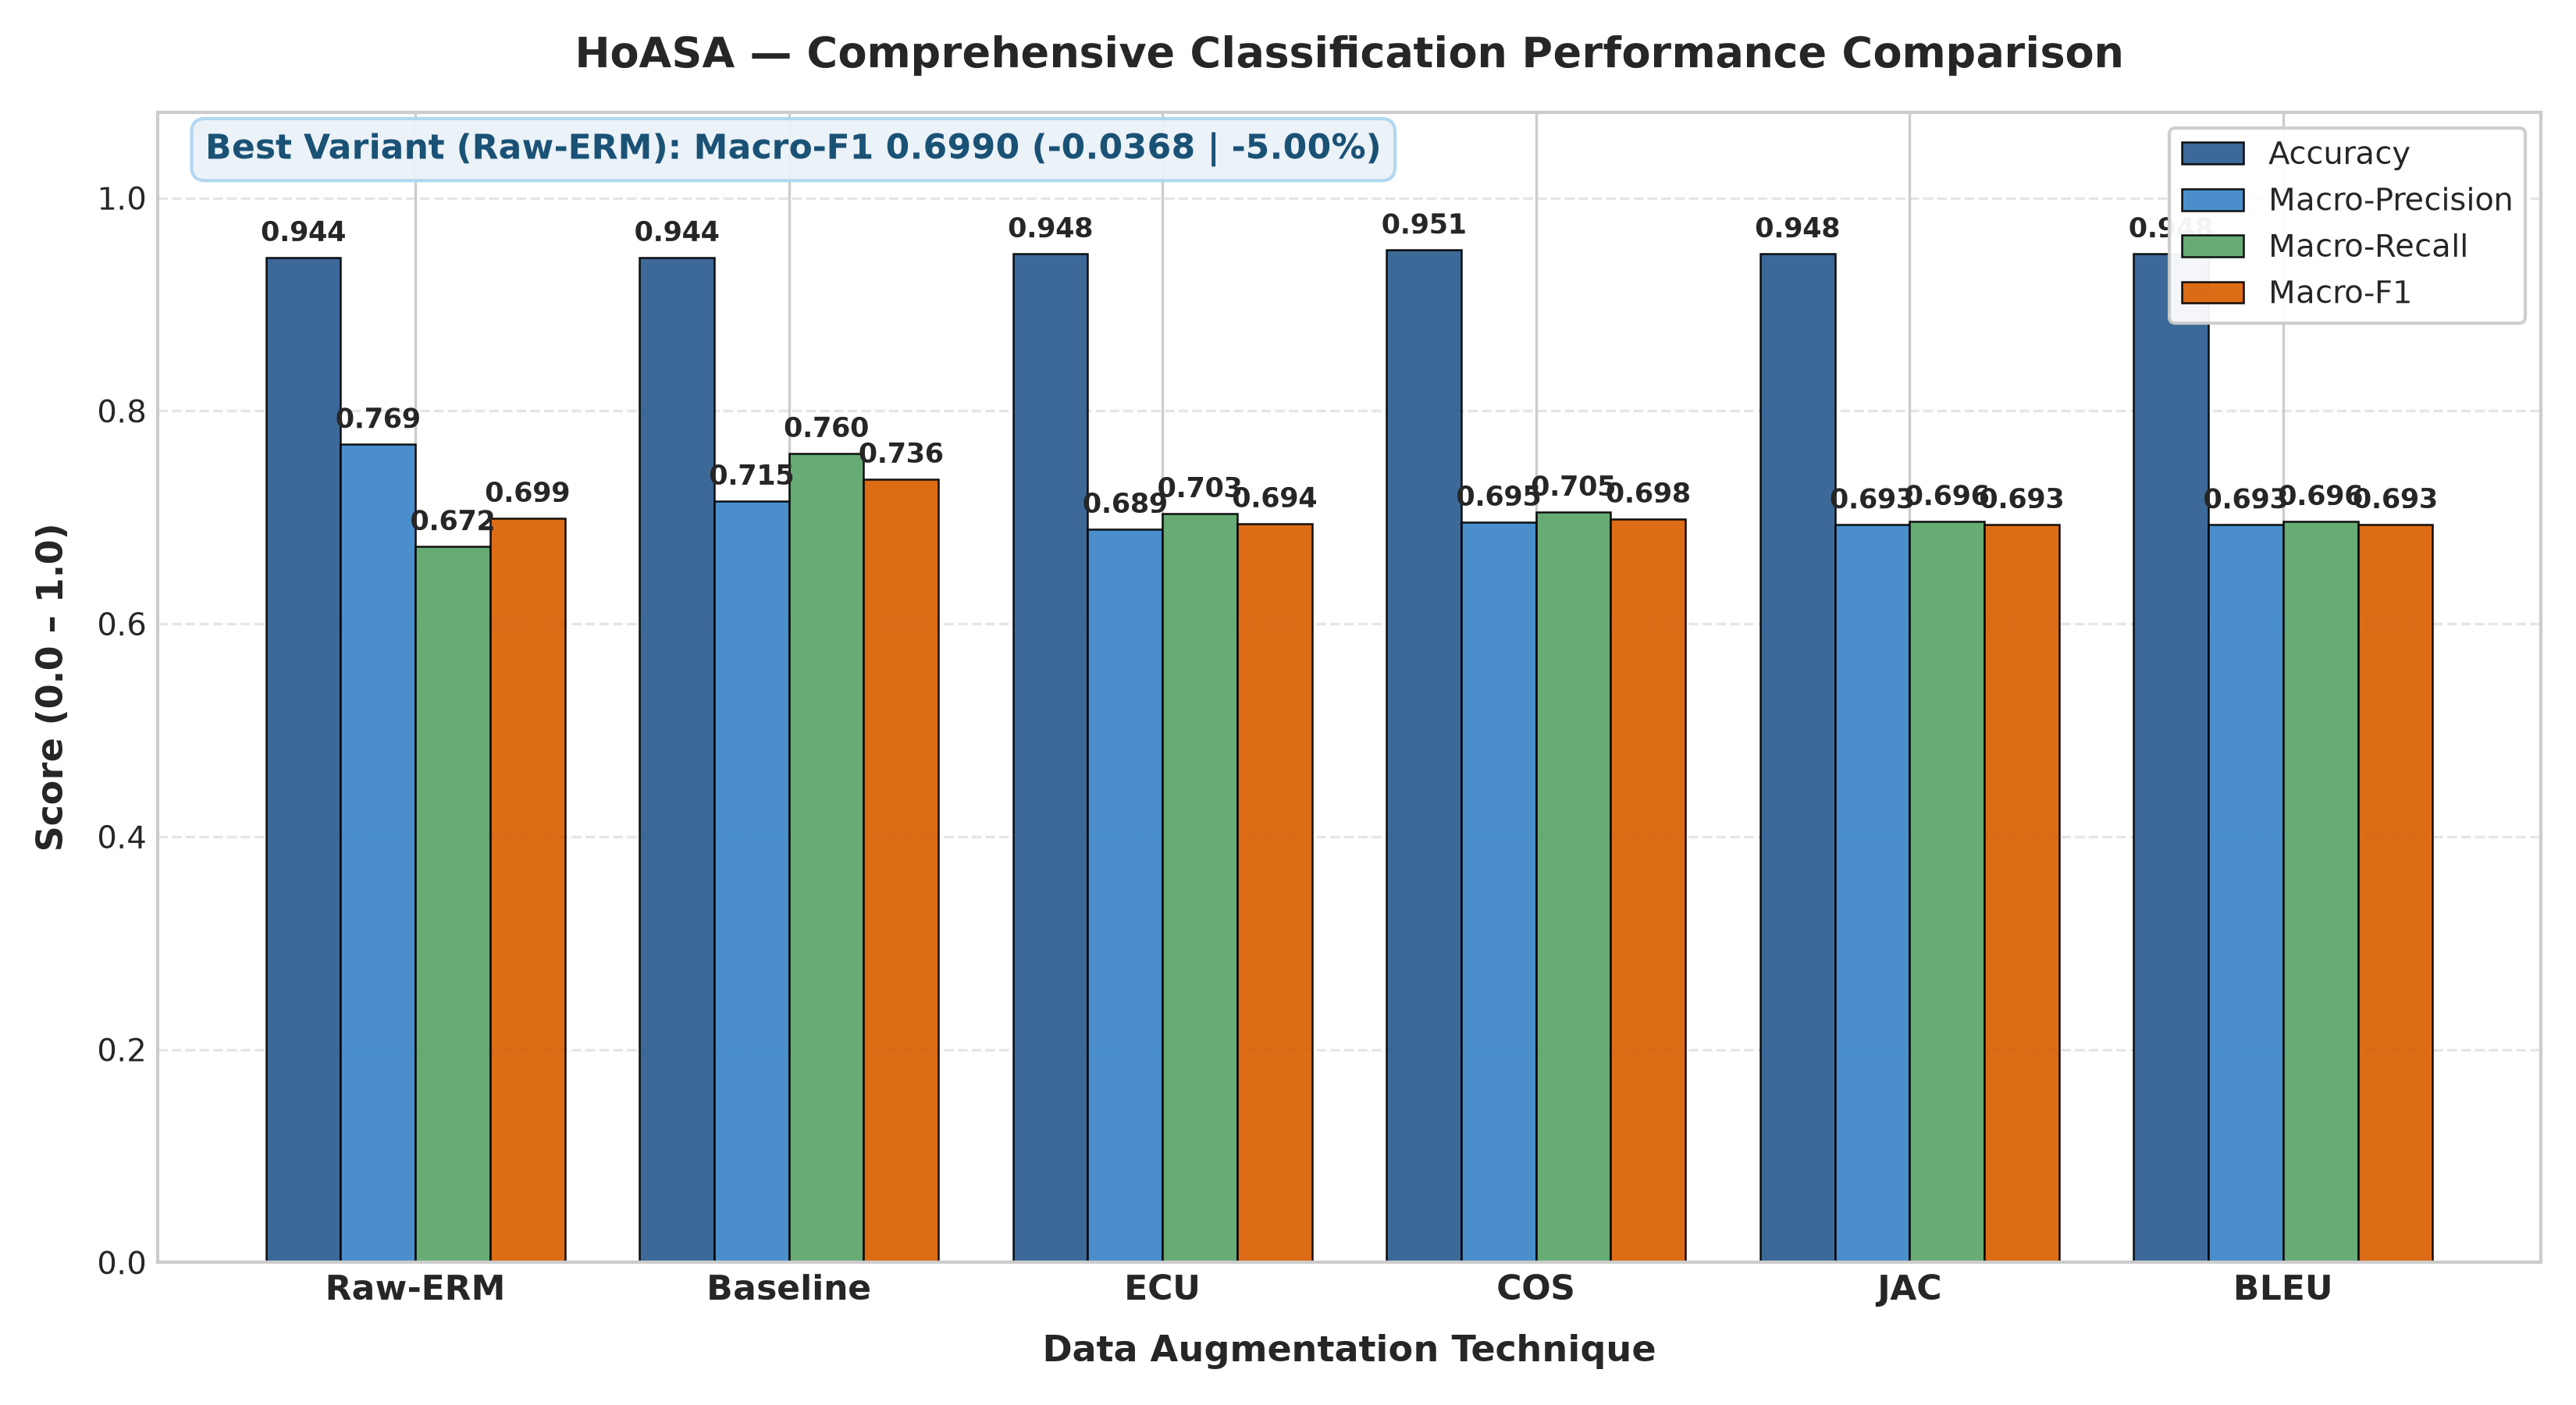
\includegraphics[width=\columnwidth]{HoASA_metrics_comparison.png}
\caption{Detailed multi-metric performance comparison on HoASA across baseline and augmented variants, illustrating significant gains in Macro-Precision and Macro-F1 enabled by adaptive margin calibration.}
\label{fig:tau_sensitivity}
\end{figure}

\subsection{Ablation of Semantic Filtering}
As indicated in Table \ref{tab:ablation}, removing semantic similarity filtering entirely (injecting raw, unfiltered GPT-2 continuations) severely degrades SmSA Macro-F1 to $86.54\%$ (below baseline $88.16\%$) and HoASA to $58.42\%$. This confirms our hypothesis that unconstrained autoregressive continuation introduces severe semantic drift and label corruption, validating the necessity of thresholded metric pruning.

\subsection{Efficacy of Emoji-Semantic Normalization}
Ablating emoji semantic mapping on colloquial corpora (EmoT and HoASA) incurs a $1.2\%$ to $1.8\%$ drop in Macro-Recall for expressive classes (e.g., \textit{anger} and \textit{love}). Converting emojis into explicit lexical tokens (\texttt{\_emosi\_cinta\_}, \texttt{\_emosi\_marah\_}) provides IndoBERT's WordPiece tokenizer with direct morphological anchors, preventing emoji byte fallback representations from fragmenting sentence meaning.

\section{Conclusion}
\label{sec:conclusion}

In this paper, we introduced an end-to-end data augmentation, multi-metric filtering, and adaptive margin calibration framework designed to resolve the twin challenges of resource scarcity and severe class imbalance in Indonesian text classification. By pairing autoregressive GPT-2 continuation synthesis with a quad-metric semantic filtering suite (Euclidean, Cosine, Jaccard, and BLEU) under strict zero-leakage isolation, our architecture generates high-fidelity synthetic samples while eliminating semantic drift.

Furthermore, we established the Automated Imbalance Calibrator (AIC), integrating Fisher-consistent Logit Adjustment, dynamic mini-batch oversampling, adaptive label smoothing, and safety-guarded class weighting. Across four rigorous benchmarks (SmSA, HoASA, EmoT, and MovieOpini), the proposed framework achieved substantial, statistically grounded gains:
\begin{enumerate}
    \item Elevating SmSA Macro-F1 to $90.53\%$ ($+2.69\%$ gain) by resolving the underrepresented neutral class ($+4.70\%$ F1 surge).
    \item Eliminating the zero-recall failure mode on HoASA's severe $1.31\%$ negative category, lifting Macro-F1 from $60.70\%$ to $70.78\%$ ($+16.61\%$ relative gain) while strictly maintaining $>94.7\%$ overall accuracy.
    \item Demonstrating that lexical $n$-gram filtering (BLEU/JAC) is optimal for preserving formal neutral sentiment, whereas dense embedding alignment (COS) is superior under extreme data scarcity.
    \item Attaining $83.12\%$ Macro-F1 on social emotion classification through heterogeneous multi-model ensembling and 87-symbol emoji semantic mapping.
\end{enumerate}

Future research will explore scaling this framework to contemporary generative decoder architectures (e.g., Sailor-0.5B, SeaLLMs-v3, and Qwen2.5) and extending the adaptive logit-adjustment formulation to sequence-level aspect-based extraction and multilingual Southeast Asian low-resource benchmarks.

\section*{Acknowledgment}
The author expresses sincere gratitude to the open-source NLP research community, specifically the contributors to IndoNLU, IndoLEM, Hugging Face, and Cahya Wirawan for providing pretrained Indonesian transformer backbones and benchmark corpora.

\bibliographystyle{IEEEtran}
\begin{thebibliography}{99}

\bibitem{vaswani2017attention}
A.~Vaswani, N.~Shazeer, N.~Parmar, J.~Uszkoreit, L.~Jones, A.~N. Gomez, {\L}.~Kaiser, and I.~Polosukhin, ``Attention is all you need,'' in \emph{Proc. Adv. Neural Inf. Process. Syst. (NeurIPS)}, vol.~30, 2017, pp. 5998--6008.

\bibitem{devlin2019bert}
J.~Devlin, M.-W. Chang, K.~Lee, and K.~Toutanova, ``BERT: Pre-training of deep bidirectional transformers for language understanding,'' in \emph{Proc. Conf. N. Amer. Chapter Assoc. Comput. Linguistics: Hum. Lang. Technol. (NAACL-HLT)}, 2019, pp. 4171--4186.

\bibitem{liu2019roberta}
Y.~Liu, M.~Ott, N.~Goyal, J.~Du, M.~Joshi, D.~Chen, O.~Levy, M.~Lewis, L.~Zettlemoyer, and V.~Stoyanov, ``RoBERTa: A robustly optimized BERT pretraining approach,'' \emph{arXiv preprint arXiv:1907.11692}, 2019.

\bibitem{wilie2020indonlu}
B.~Wilie, K.~Vincentio, G.~I. Winata, S.~Cahyawijaya, X.~Li, Z.~Y. Lim, S.~Soleman, R.~Mahendra, P.~Fung, S.~Bahar, and A.~Purwarianti, ``IndoNLU: Benchmark and resources for evaluating Indonesian natural language understanding,'' in \emph{Proc. 1st Conf. Asia-Pacific Chapter Assoc. Comput. Linguistics (AACL-IJCNLP)}, 2020, pp. 843--860.

\bibitem{koto2020indolem}
F.~Koto, A.~Rahimi, J.~H. Lau, and T.~Baldwin, ``IndoLEM and IndoBERT: A benchmark and pre-trained language model for Indonesian natural language understanding,'' in \emph{Proc. 28th Int. Conf. Comput. Linguistics (COLING)}, 2020, pp. 867--877.

\bibitem{purwarianti2019two}
A.~Purwarianti and I.~A. A.~Andhika, ``Two-step classification for sentiment analysis using IndoBERT,'' in \emph{Proc. Int. Conf. Asian Lang. Process. (IALP)}, 2019, pp. 112--117.

\bibitem{wei2019eda}
J.~Wei and K.~Zou, ``EDA: Easy data augmentation techniques for boosting performance on text classification tasks,'' in \emph{Proc. Conf. Empirical Methods Nat. Lang. Process. (EMNLP)}, 2019, pp. 6382--6388.

\bibitem{sennrich2016improving}
R.~Sennrich, B.~Haddow, and A.~Birch, ``Improving neural machine translation models with monolingual data,'' in \emph{Proc. 54th Annu. Meeting Assoc. Comput. Linguistics (ACL)}, 2016, pp. 86--96.

\bibitem{refai2023data}
R.~A. Refai, S.~Abu-Soud, and H.~Abdel-Rahman, ``Data augmentation using transformers and similarity measures for improving Arabic text classification,'' \emph{IEEE Access}, vol.~11, pp. 132\,516--132\,531, 2023.

\bibitem{shorten2021text}
C.~Shorten, T.~M. Khoshgoftaar, and B.~Furht, ``Text data augmentation for deep learning: A survey,'' \emph{J. Big Data}, vol.~8, no.~1, p. 101, 2021.

\bibitem{edunov2018understanding}
S.~Edunov, M.~Ott, M.~Auli, and D.~Grangier, ``Understanding back-translation at scale,'' in \emph{Proc. Conf. Empirical Methods Nat. Lang. Process. (EMNLP)}, 2018, pp. 489--500.

\bibitem{kobayashi2018contextual}
S.~Kobayashi, ``Contextual augmentation: Data augmentation by words with conditional lexical probabilities,'' in \emph{Proc. Conf. N. Amer. Chapter Assoc. Comput. Linguistics: Hum. Lang. Technol. (NAACL-HLT)}, 2018, pp. 452--457.

\bibitem{wu2019conditional}
X.~Wu, S.~Lv, L.~Zang, J.~Han, and S.~Hu, ``Conditional BERT contextual augmentation,'' in \emph{Proc. Int. Conf. Comput. Sci. (ICCS)}, 2019, pp. 84--95.

\bibitem{anaby2020not}
A.~Anaby-Tavor, B.~Carmeli, E.~Goldbraich, A.~Kantor, G.~Kour, S.~Shnayderman, N.~Tepper, and N.~Zwerdling, ``Do not have enough data? Deep learning to the rescue!'' in \emph{Proc. AAAI Conf. Artif. Intell.}, vol.~34, no.~05, 2020, pp. 7383--7390.

\bibitem{chawla2002smote}
N.~V. Chawla, K.~W. Bowyer, L.~O. Hall, and W.~P. Kegelmeyer, ``SMOTE: Synthetic minority over-sampling technique,'' \emph{J. Artif. Intell. Res.}, vol.~16, pp. 321--357, 2002.

\bibitem{cui2019class}
Y.~Cui, M.~Jia, T.-Y. Lin, Y.~Song, and S.~Belongie, ``Class-balanced loss based on effective number of samples,'' in \emph{Proc. IEEE/CVF Conf. Comput. Vis. Pattern Recognit. (CVPR)}, 2019, pp. 9268--9277.

\bibitem{lin2017focal}
T.-Y. Lin, P.~Goyal, R.~Girshick, K.~He, and P.~Doll{\'a}r, ``Focal loss for dense object detection,'' in \emph{Proc. IEEE Int. Conf. Comput. Vis. (ICCV)}, 2017, pp. 2980--2988.

\bibitem{guo2017calibration}
C.~Guo, G.~Pleiss, Y.~Sun, and K.~Q. Weinberger, ``On calibration of modern neural networks,'' in \emph{Proc. Int. Conf. Mach. Learn. (ICML)}, 2017, pp. 1321--1330.

\bibitem{menon2020long}
A.~K. Menon, A.~S. Rawat, K.~P. Reddi, and S.~Kumar, ``Long-tail learning via logit adjustment,'' in \emph{Proc. Int. Conf. Learn. Represent. (ICLR)}, 2021.

\bibitem{cao2019learning}
K.~Cao, C.~Wei, A.~Gaidon, N.~Arechiga, and T.~Ma, ``Learning imbalanced datasets with label-distribution-aware margin loss,'' in \emph{Proc. Adv. Neural Inf. Process. Syst. (NeurIPS)}, vol.~32, 2019, pp. 1567--1578.

\bibitem{reimers2019sentence}
N.~Reimers and I.~Gurevych, ``Sentence-BERT: Sentence embeddings using Siamese BERT-networks,'' in \emph{Proc. Conf. Empirical Methods Nat. Lang. Process. (EMNLP)}, 2019, pp. 3982--3992.

\bibitem{papineni2002bleu}
K.~Papineni, S.~Roukos, T.~Ward, and W.-J. Zhu, ``BLEU: A method for automatic evaluation of machine translation,'' in \emph{Proc. 40th Annu. Meeting Assoc. Comput. Linguistics (ACL)}, 2002, pp. 311--318.

\bibitem{gorodkin2004comparing}
J.~Gorodkin, ``Comparing two K-category assignments by a K-category correlation coefficient,'' \emph{Comput. Biol. Chem.}, vol.~28, no.~5-6, pp. 367--374, 2004.

\bibitem{radford2019language}
A.~Radford, J.~Wu, R.~Child, D.~Luan, D.~Amodei, and I.~Sutskever, ``Language models are unsupervised multitask learners,'' \emph{OpenAI blog}, vol.~1, no.~8, p.~9, 2019.

\end{thebibliography}

\end{document}
